\subsubsection*{Partie I.}
\begin{figure}
	\begin{center}
	\input{Cconi2_1.pdf_t}
	\end{center}
\caption{I.1. Cas $0<c<a$.}
\label{fig:Cconi2_1}
\end{figure} 
\begin{figure}
	\begin{center}
	\input{Cconi2_2.pdf_t}
	\end{center}
\caption{I.1.Cas $0<c=a$.}
\label{fig:Cconi2_2}
\end{figure} 
\begin{figure}
	\begin{center}
	\input{Cconi2_3.pdf_t}
	\end{center}
\caption{I.1. Cas $0<a<c$.}
\label{fig:Cconi2_3}
\end{figure} 

\begin{enumerate}
 \item Voir Fig. \ref{fig:Cconi2_1}, Fig. \ref{fig:Cconi2_2}, Fig.\ref{fig:Cconi2_3} .
 \item Lorsque $c=a$, comme $B$ et $C_\theta$ sont sur le même cercle (Fig. 2.) de centre $A$, l'intersection de la médiatrice de $[BC_\theta]$ avec la droite $(AC_\theta)$ est toujours $A$.
\begin{displaymath}
 \mathcal C = \{A\}
\end{displaymath}
\item Les calculs sont évidents :
\begin{align*}
 z(A)=0 &,& z(B)=2c &,& z(C_\theta)=2ce^{i\theta} &,& z(H_\theta)=c+ae^{i\theta} 
\end{align*}
Lorsque $\theta$ varie, le point $H_\theta$ décrit le cercle de centre de point de coordonnées $(c,0)$ et de rayon $a$.
\item 
\begin{enumerate}
 \item Comme $M_\theta$ est sur la droite $(AC_\theta)$, il existe un réel $\lambda$ tel que
\begin{displaymath}
 z(M_\theta) = \lambda e^{i\theta}
\end{displaymath}
\item \'Ecrivons l'orthogonalité de $\overrightarrow{H_\theta M_\theta}$ et $\overrightarrow{BC_\theta}$ avec les affixes complexes :
\begin{displaymath}
 \frac{\lambda e^{i\theta} -c - a e^{i\theta}}{2ae^{i\theta}-2c} \in i\R
\end{displaymath}
Le $2$ qui se met en facteur au dénominateur ne change pas la condition d'être imaginaire pur. On le fait donc disparaitre. On multiplie par $e^{-i\theta}$ en haut et en bas. La condition devient :
\begin{displaymath}
 \frac{\lambda -a -c e^{-i\theta} }{a-ce^{-i\theta}} \in i\R
\end{displaymath}
Si on multiplie en haut et en bas par la quantité conjuguée du dénominateur, celui ci devient un réel sctrictement positif et peut donc disparaitre de la condition. On obtient alors :
\begin{displaymath}
 (\lambda -a -c e^{-i\theta})(a-ce^{i\theta}) \in i\R
\end{displaymath}
\item Le point $M_\theta$ existe lorsque la médiatrice de $BC_\theta$ coupe $AC_\theta$. Le point n'est pas correctement défini lorsque ces droites sont parallèles c'est à dire lorsque le triangle $AC_\theta B$ est rectangle en $C_\theta$. Cela ne peut se produire que si 
\begin{align*}
 c>a & & \cos \theta =\dfrac{a}{c}
\end{align*}
Il existe donc un point $M_\theta$
\begin{itemize}
 \item pour tous les $\theta$ lorsque $c<a$
\item pour tous les $\theta$ autres que $\theta_0$ et $-\theta_0$ lorsque $c>a$.
\end{itemize}
Calculons $M_\theta$ dans ces cas.\newline
D'après b., l'affixe de $M_\theta$ est de la forme $\lambda e^{i\theta}$ avec $\lambda$ vérifiant :
\begin{displaymath}
 (\lambda -a-ce^{i\theta})(a-ce^{i\theta})\in i\R
\end{displaymath}
\'Ecrivons que la partie rélle est nulle :
\begin{displaymath}
 (\lambda - a-c \cos \theta)(a-c \cos \theta)-(c\sin \theta)(-c\sin \theta)=0\Leftrightarrow
\lambda = \dfrac{a^2-c^2}{a-c\cos \theta}
\end{displaymath}
\end{enumerate}
\item Lorsque $c<a$, pour tous les $\theta$ : $\lambda >0$.\newline
Lorsque $a<c$, on peut former le tableau :
\begin{displaymath}
\begin{array}{ccccccc}
 -\pi &   & -\theta_0 &   & \theta_0 &   & \pi \\ \hline
      & - &   \Vert  & + & \Vert    & - &  
\end{array}
 \end{displaymath}

\end{enumerate}
\subsubsection*{Partie II.}
\begin{figure}[ht]
 \centering
\input{Cconi2_4.pdf_t}
\caption{Définition bifocale : ellipse $c<a$}
\label{fig:Cconi2_4}
\end{figure}
\begin{figure}[ht]
 \centering
\input{Cconi2_5.pdf_t}
\caption{Définition bifocale : branches d'hyperbole $a<c$}
\label{fig:Cconi2_5}
\end{figure}
\begin{enumerate}
 \item Par construction, le point $M_\theta$ est sur la médiatrice de $BC_\theta$ donc $M_\theta C_\theta=M_\theta B$. 
\item D'après les questions précédentes, l'affixe de $M_\theta$ est $\lambda e^{i\theta}$ avec 
\begin{displaymath}
 \lambda = \dfrac{a^2-c^2}{a-\cos \theta}
\end{displaymath}
L'ordre dans lequel sont placés les points alignés $A$, $M_\theta$, $C_\theta$ dépend du signe de $\lambda$ et de $2a-\lambda$.\newline
Dans le cas où $c<a$, ces deux réels sont strictement positifs. Les points $A$, $M_\theta$, $C_\theta$ sont alignés dans cet ordre avec
\begin{displaymath}
 AM_\theta + BM_\theta = AM_\theta + M_\theta C_\theta = 2a
\end{displaymath}
Le point $M_\theta$ décrit alors une ellipse de foyers $A$ et $B$ et de grand axe $2a$ (Fig.\ref{fig:Cconi2_4})\newline
Lorsque $a<c$, le point $M_\theta$ décrit les branches d'une hyperbole de foyers $A$ et $B$ (Fig. \ref{fig:Cconi2_5}). Le détail est présenté dans un tableau:
\begin{displaymath}
\begin{array}{cccccccc}
             &-\pi &   & -\theta_0 &   & \theta_0 &   & \pi \\ \hline
     \lambda & |   & - &   \Vert  & + & \Vert    & - &  \\ \hline
 2a- \lambda & |   & + &   \Vert  & - & \Vert    & + &  \\ \hline
\text{alignement} & |   & MAC &   \Vert  & ACM & \Vert    & MAC &  \\ \hline
2a= & |   & MB -MA &   \Vert  & MA-MB & \Vert &  MB -MA &  
\end{array}
 \end{displaymath}
\end{enumerate}

\begin{figure}[ht]
 \centering
 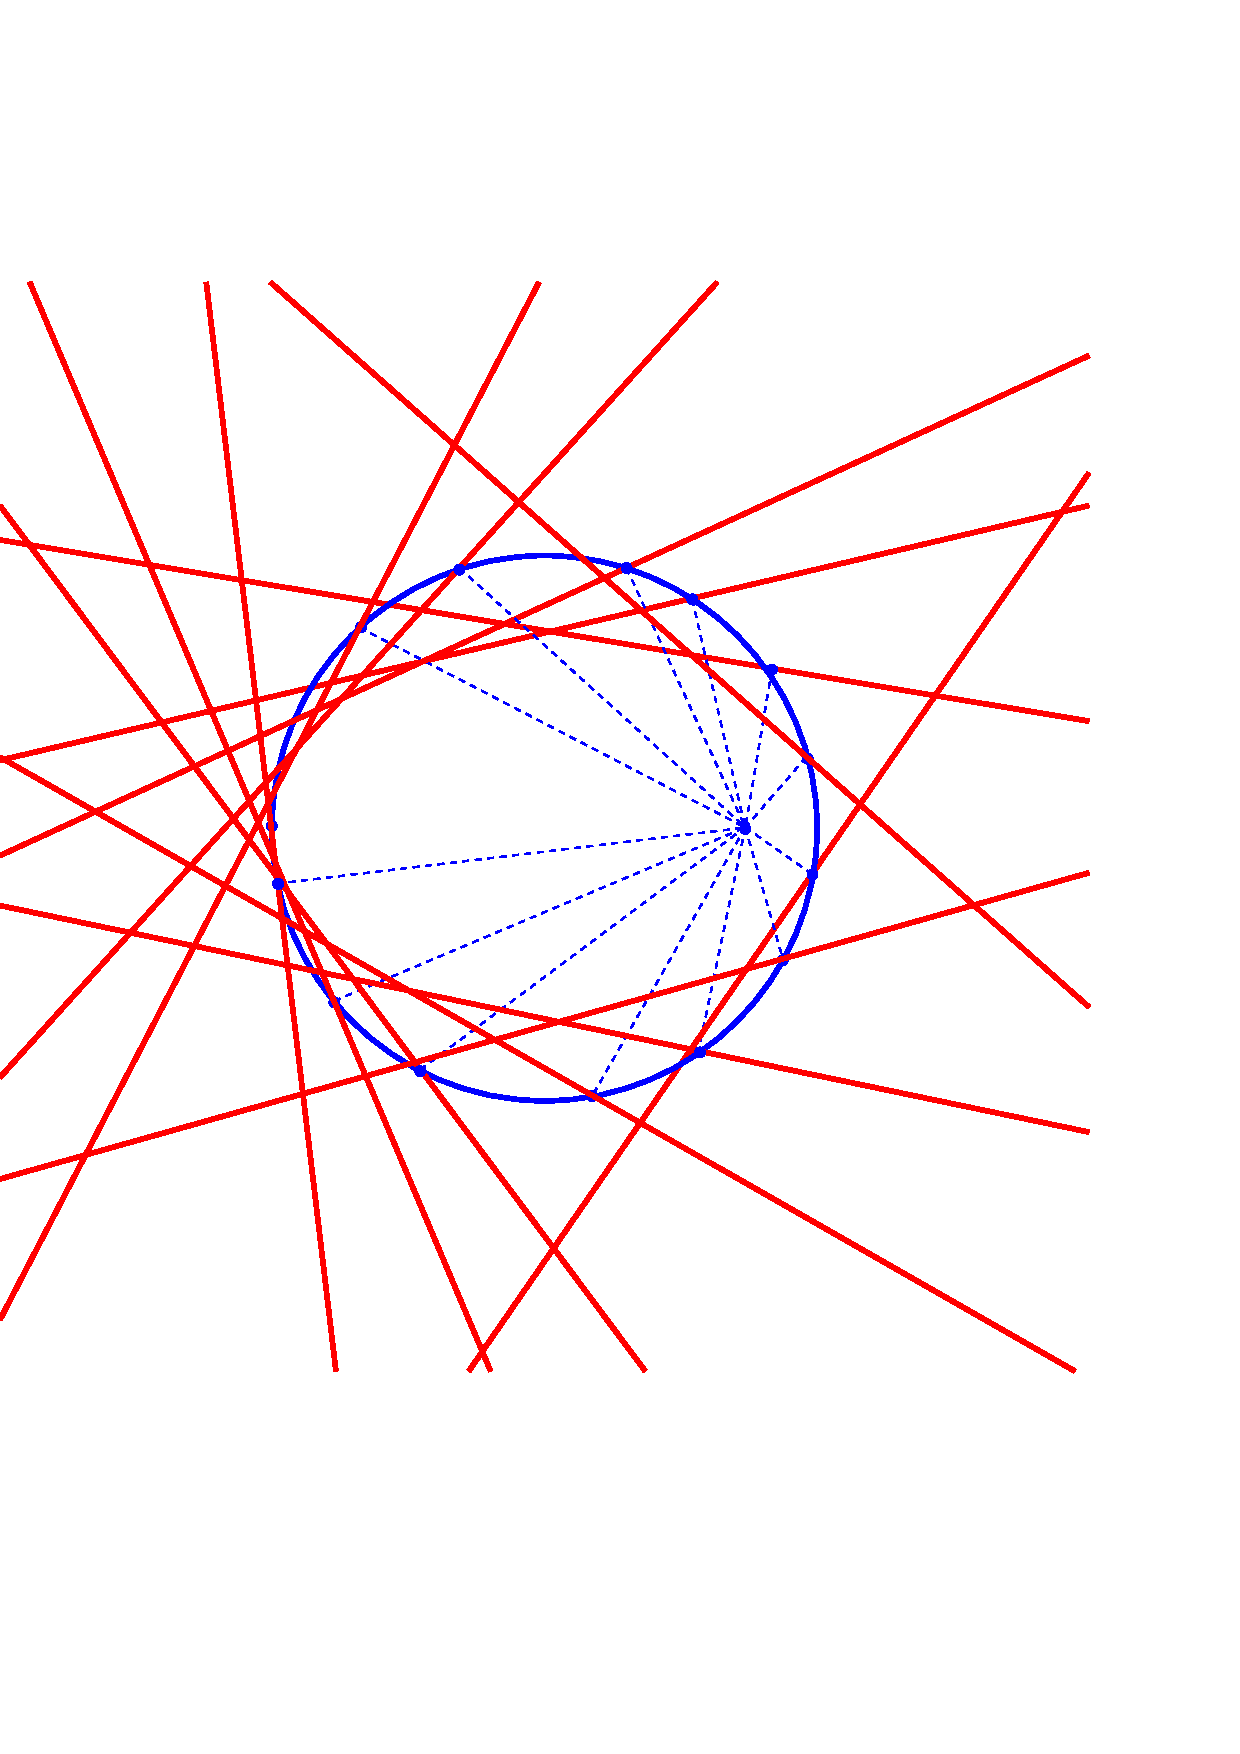
\includegraphics[width=7.5cm]{Cconi2_7.pdf}
 % Cconi2_7.pdf: 595x842 pixel, 72dpi, 20.99x29.70 cm, bb=0 0 595 842
\caption{III.3.b Enveloppe d'une famille de droites}
\label{fig:Cconi2_7}
\end{figure}
\subsubsection*{Partie III.}
\begin{enumerate}
 \item L'intersection des deux droites est régie par un système de deux équations linéaires dont le déterminant est 
\begin{displaymath}
 U(t)V^\prime(t)-U^\prime(t)V(t)\neq 0
\end{displaymath}
Ce système admet donc pour chaque $t$ un unique couple solution. On le note $(a(t),b(t))$.
\item Il ne faut \emph{surtout pas} chercher à préciser lescoordonnées $(a(t),b(t))$ du point $f(t)$.  \'Ecrivons que $f(t)\in \Delta_t$ puis dérivons cette relation :
\begin{eqnarray*}
 0&=& U(t)a(t)+V(t)b(t)+W(t) \\
0 &=& \left( U^\prime(t)a(t)+V^\prime(t)b(t)+W^\prime(t)\right)  + U(t)a^\prime(t)+V(t)b^\prime(t)
\end{eqnarray*}
La parenthèse est nulle car $f(t)\in \Delta^\prime _t$. Le reste de la relation traduit l'orthogonalité de $\overrightarrow{f^\prime}(t)$ avec le vecteur de coordonnées $(U(t),V(t))$. Or ce vecteur est normal à $\Delta_t$ (d'après son équation), on en déduit donc que $\overrightarrow{f^\prime}(t)$ est dans la direction de $\Delta_t$ ce qui assure que c'est la tangente car elle contient $f(t)$.
\item
\begin{enumerate}
 \item Pour former l'équation de $\Delta_t$, on écrit la nullité du produit scalaire des vecteurs de coordonnées
\begin{align*}
 \begin{pmatrix}
  x-R\cos t \\ y-R\sin t
 \end{pmatrix}
& &
\begin{pmatrix}
 R\cos t -s \\ R\sin t
\end{pmatrix}
\end{align*}
On obtient après calculs :
\begin{displaymath}
 \text{équation de $\Delta_t$ } : 
(R\cos t -s)x+R\sin t y -R^2+Rs\cos t =0
\end{displaymath}

\item Les coordonnées de $f(t)$ sont les solutions du système
\begin{displaymath}
 \left\lbrace 
\begin{aligned}
 (R\cos t -s)x+R\sin t y -R^2+Rs\cos t =& 0\\
 -R\sin t x +R \cos t y -Rs\sin t =&0
\end{aligned}
\right. 
\end{displaymath}
 Que l'on résoud (après division de la deuxième équation par $-R$) à l'aide des formules de Cramer. On obtient
\begin{align*}
 x=R\,\dfrac{s-R\cos t}{s\cos t -R} & & y=(s^2-R^2)\dfrac{\sin t}{s\cos t -R}
\end{align*}
Sur la figure \ref{fig:Cconi2_7}, on voit se dessiner une ellipse.
\end{enumerate}

\end{enumerate}

\subsubsection*{Partie IV.}
\begin{enumerate}
 \item Par définition, $\mathcal D_\theta$ est la médiatrice de $B$ et de $C_\theta$. Pour obtenir l'équation, écrivons l'égalité des carrés des distance à ces deux points
\begin{displaymath}
 (x-2a\cos \theta)^2+(y-2a\sin \theta)^2=(x-2c)^2+y^2
\end{displaymath}
après simplifications 
\begin{align*}
 \text{équation de $\mathcal D_\theta$ : } & &
(c-a\cos \theta)x - a\sin\theta y +a^2-c^2 =0
\end{align*}

\item On forme l'équation de $\mathcal D'_\theta$ en dérivant les coefficients
\begin{displaymath}
 a\sin \theta x-a\cos \theta y =0
\end{displaymath}
On résout le système constitué par les deux équations avec les formules de Cramer:
\begin{align*}
 \begin{vmatrix}
  c-a\cos\theta & -a\sin \theta \\
  \sin \theta & -\cos\theta
 \end{vmatrix} =& -c\cos \theta +a \\
\begin{vmatrix}
 -a^2+c^2 & -a\sin \theta \\
0 & -\cos \theta
\end{vmatrix}=&(a^2-c^2)\cos\theta \\
\begin{vmatrix}
 c-a\cos\theta &-a^2+c^2 \\
\sin \theta & 0
\end{vmatrix}=&(a^2-c^2)\sin \theta
\end{align*}
Les coordonnées du point d'intersection sont donc
\begin{displaymath}
 \left( \dfrac{a^2-c^2}{a-c\cos\theta}\cos \theta , \dfrac{a^2-c^2}{a-c\cos\theta}\sin \theta \right) 
\end{displaymath}
ce qui correspond bien à l'affixe complexe de $M_\theta$ trouvée en I. D'après la partie III, la courbe $\mathcal C$ est l'enveloppe des droites $\mathcal D_\theta$. Chacune de ces droites est donc tangente à $\mathcal C$ en $M_\theta$.
\item La distance d'un point à une droite s'obtient en utilisant l'équation de cette droite (obtenue en 1.)
\begin{displaymath}
 d(A,\mathcal D_\theta)d(B,\mathcal D_\theta)
=\dfrac{(a^2-c^2)\left((c-a\cos\theta)2c+a^2-c^2 \right) }{(c-a\cos\theta)^2+a^2\sin^2\theta}
=a^2-c^2
\end{displaymath}

\item Comme $\mathcal D_\theta$ est tangente à la conique et orthogonale à $C_\theta B$, la projection orthogonale sur la tangente en $M_\theta$ est $H_\theta$. L'affixe de ce point est 
\begin{displaymath}
 c+ae^{i\theta}
\end{displaymath}
Il décrit un cercle de centre $B$ et de rayon $a$. La podaire d'un foyer sur une conique (ellipse ou hyperbole) est donc un cercle. Le cas d'une parabole est examiné dans la dernière partie.
\end{enumerate}

\begin{figure}[ht]
 \centering
\input{Cconi2_6.pdf_t}
\caption{Podaire d'un foyer sur une parabole}
\label{fig:Cconi2_6}
\end{figure}
\subsubsection*{Partie V.}
\begin{enumerate}
\item\begin{enumerate}
 \item Pour obtenir l'équation cartésienne de $\mathcal P$, on écrit que $M$ de coordonnées $(x,y)$ est sur $\mathcal P$ si et seulement si $d(M,\mathcal D)=MF$
\begin{displaymath}
 \vert x+\dfrac{p}{2}\vert=\sqrt{(x-\dfrac{p}{2})^2+y^2}
\Leftrightarrow
(x+\dfrac{p}{2})^2=(x-\dfrac{p}{2})^2+y^2
\Leftrightarrow
y^2=2px
\end{displaymath}
 \item Les coordonnées de $M_u$ vérifient l'équation cartésienne de la parabole.
\end{enumerate}
 
\item On connait les coordonnées de $M_u$ et de sa dérivée :
\begin{align*}
 M_u:(2pu^2,2pu) & & \overrightarrow M_u :(4pu,2p)
\end{align*}
On en déduit l'équation de la tangente en $M_u$:
\begin{align*}
\text{équation de $\mathcal T_u$ : }& &
 \begin{vmatrix}
  x-2pu^2 & 2u \\
y-2pu & 1
 \end{vmatrix}=0
\Leftrightarrow
x-2uy+2pu^2=0
\end{align*}

\item Les coordonnées de $K_u$ sont $(-\frac{p}{2},2pu)$, écrivons encore une fois les distances à la droite avec son équation:
\begin{align*}
 d(F,\mathcal T_u)=&\dfrac{\frac{p}{2}+2pu^2}{\sqrt{1+4u^2}}\\
d(K_u,\mathcal T_u)=&\dfrac{\left\vert -\frac{p}{2}-2u(2pu)+2pu^2 \right\vert}{\sqrt{1+4u^2}}
= d(F,\mathcal T_u)
\end{align*}
On en déduit que $\mathcal T_u$ est la médiatrice de $[K_u,F]$.
\item Comme $\mathcal T_u$ est la médiatrice de $[K_u,F]$, le projeté $H_u$ de $F$ sur la tangente $\mathcal T_u$ est le milieu de $[F,K_u]$. Par conséquent, comme $F$ a pour coordonnées $(\frac{p}{2},0)$, lorsque $K_u$ décrit $\mathcal D$ (d'équation $x=\frac{p}{2}$), le point $H_u$ décrit l'axe $Oy$ (Fig. \ref{fig:Cconi2_6}).
\end{enumerate}

\clearpage